\subsection{Opsummering af filtre}
\label{OpsummeringAfFiltre}
%
Baseret på dimensioneringen af de fire filtre der forstærker og de tre der dæmper kan de endelige kurver, som opnår størst linearitet mellem 20Hz og 1000Hz repræsenteres, jævnfør \autoref{fig:EndeligeFiltre}.
%
\begin{figure}[H]
	\centering
	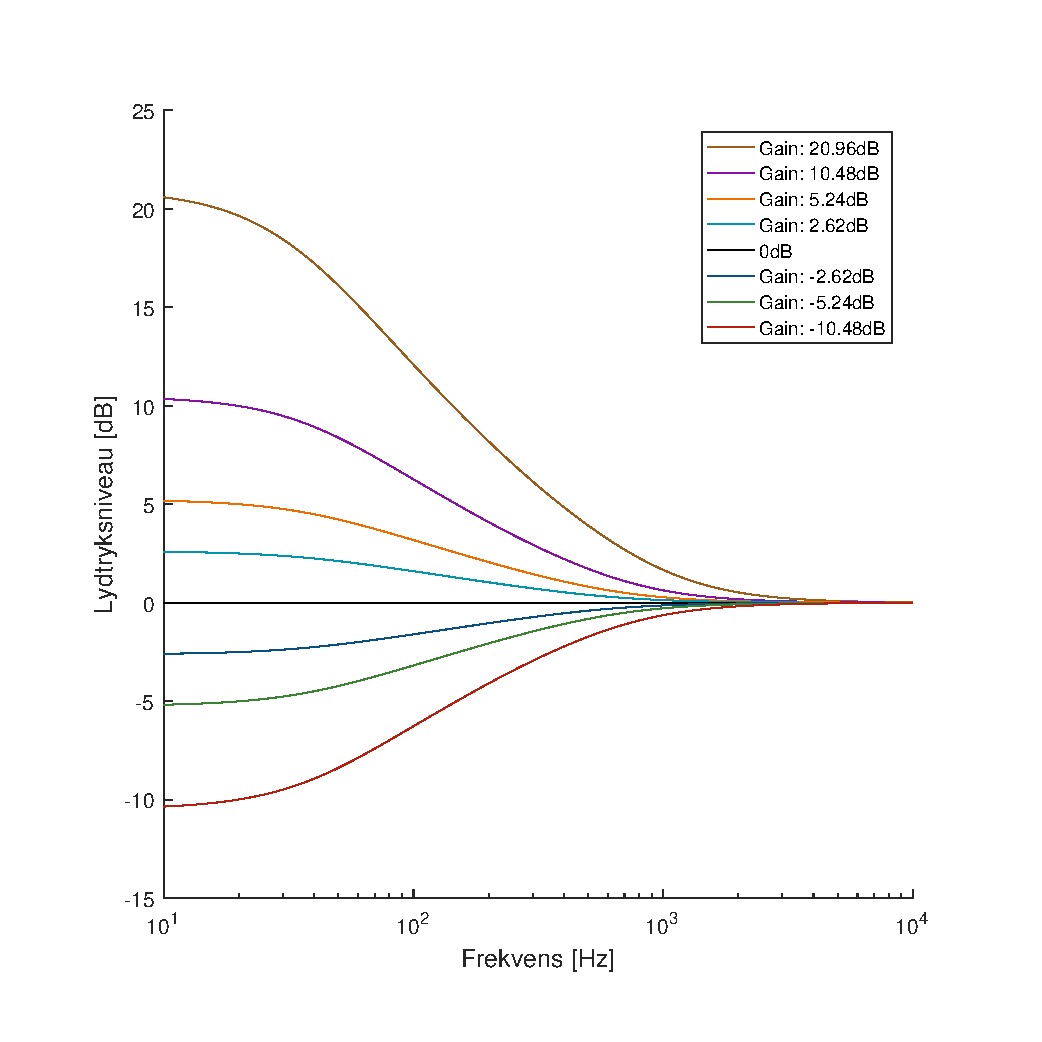
\includegraphics[resolution=300,width=\textwidth]{Figure/DesignAfFilter/EndeligeFiltre.pdf}
	\caption{Hældningerne for de fire filtre der forstærker og de tre der dæmper de lave frekvenser, hvor hver kurve repræsentere én af de syv forstærkninger i dB ved 20Hz.}
	\label{fig:EndeligeFiltre}
\end{figure}
\noindent
%
Sammenholdes kurverne på \autoref{fig:EndeligeFiltre} med resultatet af den teoretisk bedste overføringsfunktion for hver forstærkning, angivet i \autoref{tab:ForstaerkningTilDeSyvFiltre}, hvor knækket er ved præcist 20Hz, hvorfor der intet indrulningsforløb fremgår, og hældningen er lineær mellem 20Hz og 1000Hz. Data til \autoref{fig:EndeligeFiltre} forefindes i vedlagte mappe, som er navngivet: \textit{SupplerendeMateriale}
%
\begin{figure}[H]
	\centering
	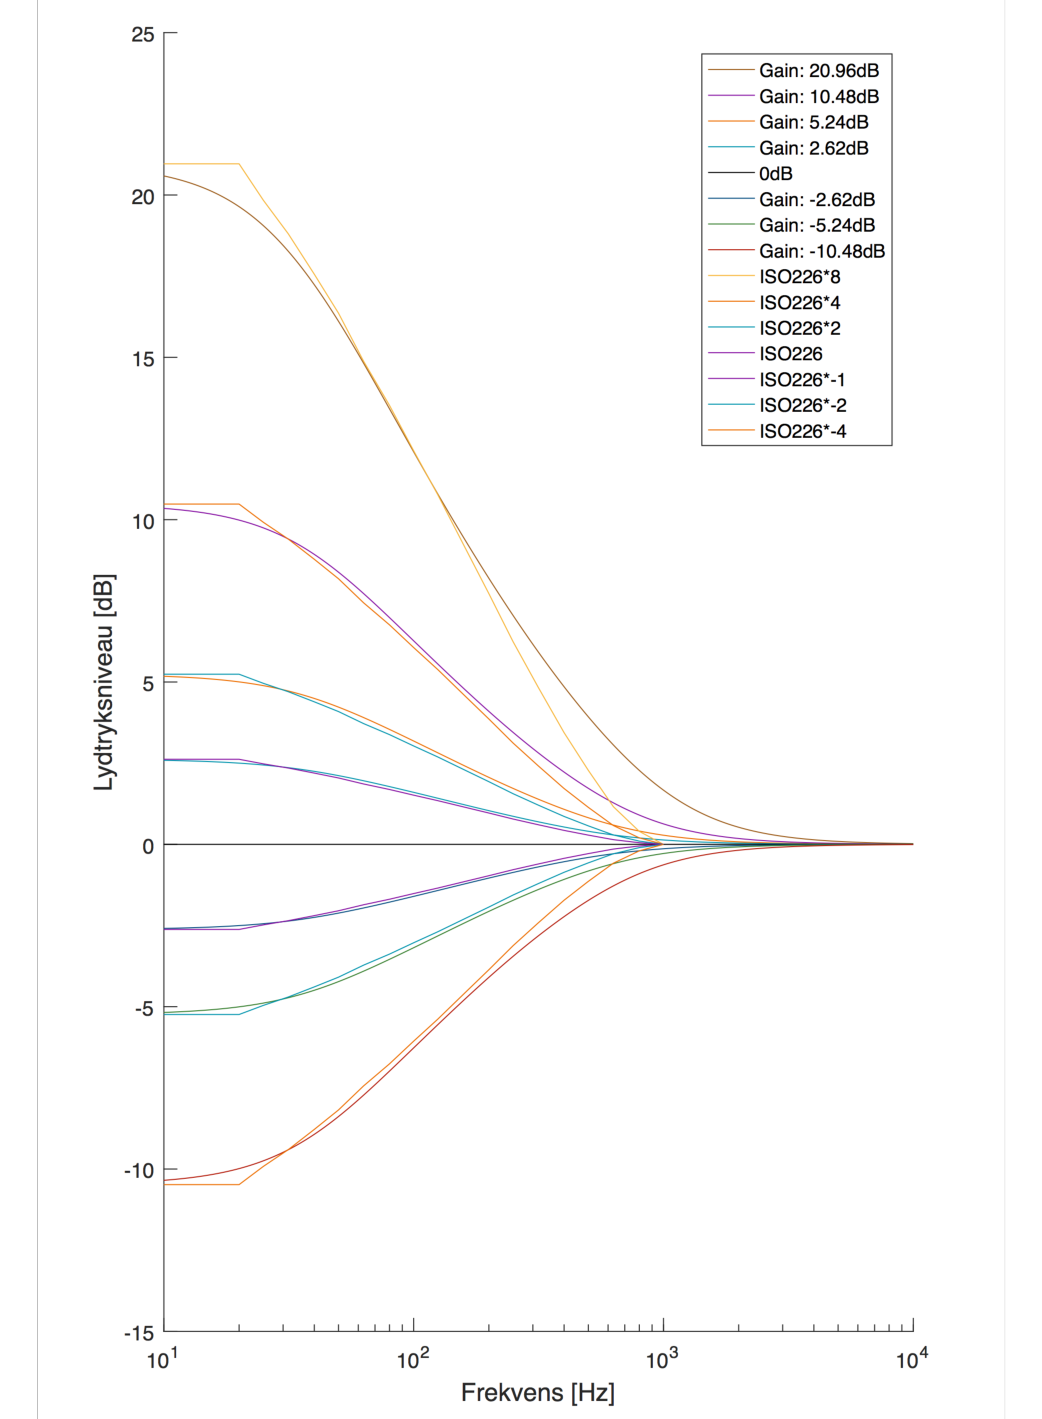
\includegraphics[resolution=300,width=\textwidth]{Figure/DesignAfFilter/EndeligeFiltreMedReferenceSHORT.pdf}
	\caption{Repræsentation af hældningerne for hvert filter sammenlignet med resultatet af den tilsvarende teoretiske bedste overføringsfunktion, hvor forstærkningen fremgår af \autoref{tab:ForstaerkningTilDeSyvFiltre}}.
	\label{fig:EndeligeFiltreMedReference}
\end{figure}
\noindent
%
På \autoref{fig:EndeligeFiltreMedReference} sammenholdes hældningerne fra hvert filter med resultatet af den tilsvarende teoretiske bedste overføringsfunktion, hvor knækket er ved præcist 20Hz, hvorfor der intet indrulningsforløb er, og hældningen er lineær mellem 20Hz og 1000Hz. Det tyder desværre på at ved en forstærkning på 20.96dB bør der foretages nogle justeringer. Disse justeringer kunne være at vælge en mindre pol $(<55Hz)$, for på den måde at forskyde kurven på x-aksen, det vil dog resultere i at kondensatorværdierne næsten vil være ens, og dermed kan det overvejes om det vil være en fordel at fjerne et RC-led. Ved at fjerne et RC-led vil det også resultere i en stejlere hældning. Selvom det er muligt at reducere afvigelsen mellem kurven: $Gain: 20.96dB$ og $ISO226*8$, gøres det ikke og det vælges at arbejde videre med $Gain: 20.96dB$, som den er beregnet.  
